\documentclass{article}

\usepackage{graphicx}
\usepackage{tikz}
\usepackage{tikzsymbols}
\usetikzlibrary{calc,patterns,shapes.geometric}
\pagestyle{empty}
\usepackage[margin=0pt]{geometry}
\geometry{papersize={14in,12in}}

\def\centerarc[#1](#2)(#3:#4:#5){\draw[#1] ($(#2)+({#5*cos(#3)},{#5*sin(#3)})$) arc (#3:#4:#5);}

\begin{document}
	\begin{figure}
		\centering
		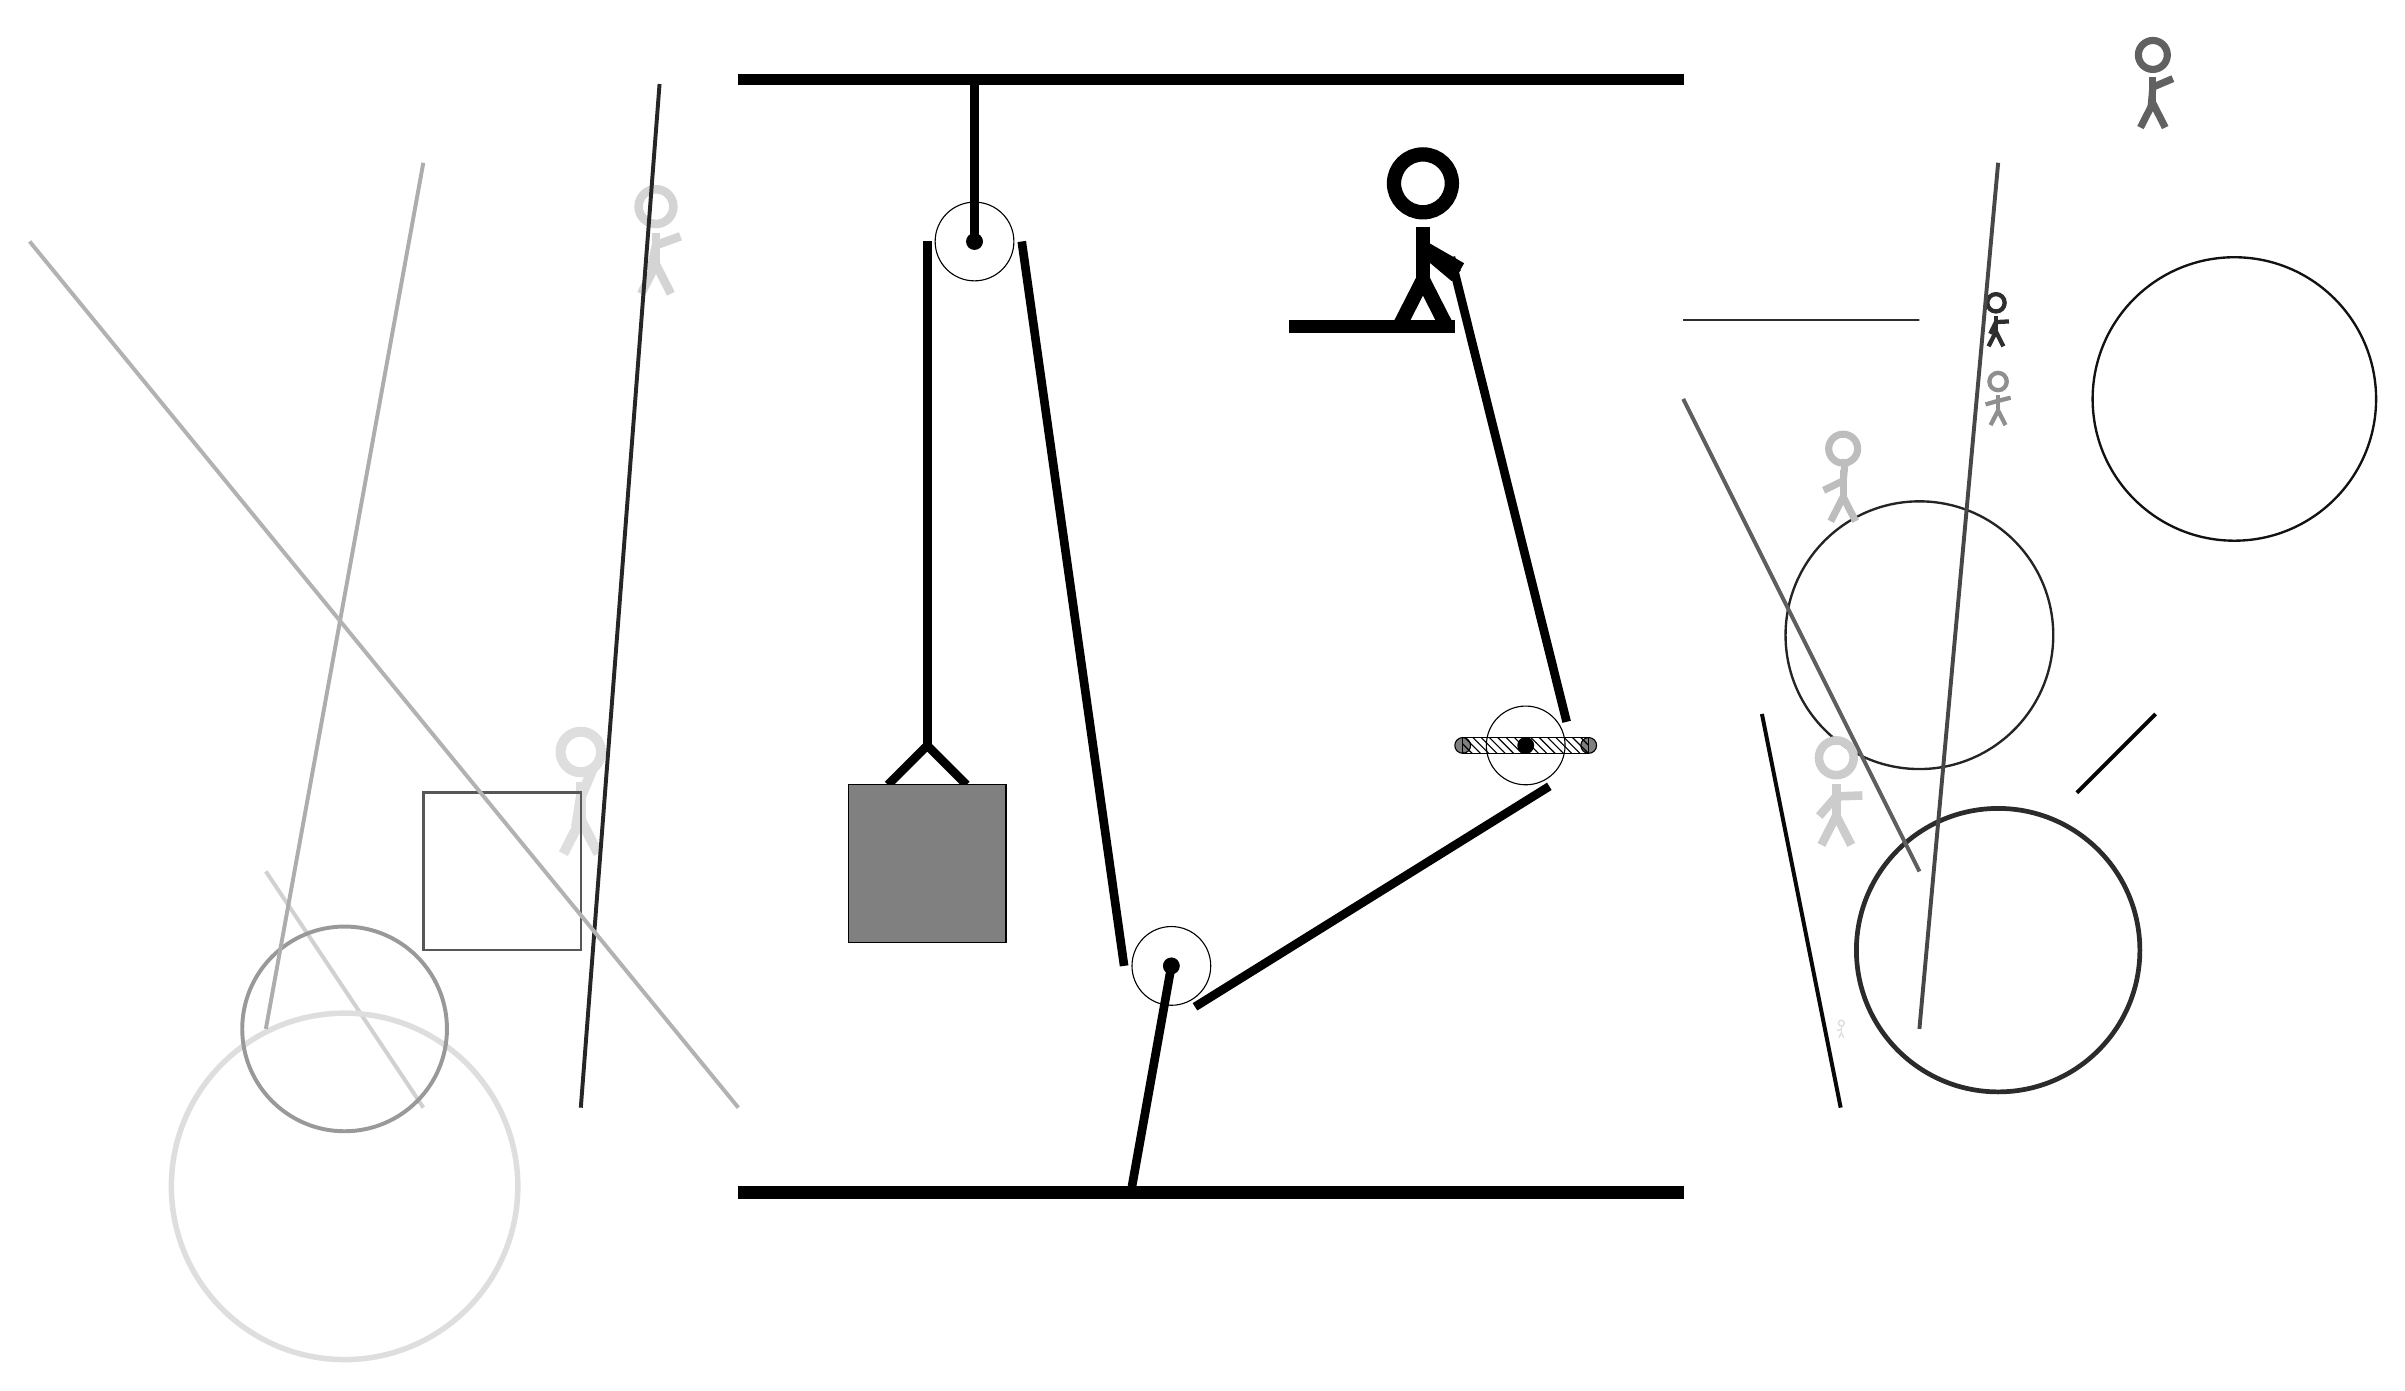
\begin{tikzpicture}
			%%%%% START %%%%%
			
			\draw[fill=black] (-2, 14) rectangle (10, 14.125);
			
			\draw (1, 12) circle (0.5);
			\draw[fill=black] (1, 12) circle (0.1);
			\draw[line width=1.1mm] (1, 14) -- (1, 12);
			
			\draw[line width=0.5mm, color=black!97](12, 1) -- (11, 6);
			
			\draw [line width=0.3mm, color=black!86](13, 7) circle (1.7);
			\node[line width=0.7mm, color=black!13] at (-4, 5) {\Strichmaxerl[7][81][67]};
			\node[line width=0.5mm, color=black!82] at (14, 11) {\Strichmaxerl[3][64][3]};
			\node[line width=0.2mm, color=black!17] at (-3, 12) {\Strichmaxerl[6][78][20]};
			
			\draw [line width=0.3mm, color=black!93](17, 10) circle (1.8);
			\draw[line width=0.5mm, color=black!85](-3, 14) -- (-4, 1);
			\draw[line width=0.5mm, color=black!99](15, 5) -- (16, 6);
			\draw[line width=0.5mm, color=black!18](-6, 1) -- (-8, 4);
			
			\node[line width=0.4mm, color=black!26] at (12, 9) {\Strichmaxerl[5][26][84]};
			\node[line width=0.7mm, color=black!13] at (12, 2) {\Strichmaxerl[1][9][84]};
			\draw[line width=0.3mm, color=black!66] (-4, 3) rectangle (-6, 5);
			\node[line width=0.2mm, color=black!62] at (16, 14) {\Strichmaxerl[5][85][23]};
			\draw [line width=0.6mm, color=black!83](14, 3) circle (1.8);
			\draw [line width=0.7mm, color=black!13](-7, 0) circle (2.2);
			\draw[line width=0.2mm, color=black!82] (10, 11) rectangle (13, 11);
			
			\draw [line width=0.5mm, color=black!40](-7, 2) circle (1.3);
			\node[line width=0.4mm, color=black!44] at (14, 10) {\Strichmaxerl[3][16][14]};
			\draw[line width=0.5mm, color=black!32](-6, 13) -- (-8, 2);
			
			\draw[line width=0.5mm, color=black!63](10, 10) -- (13, 4);
			\node[line width=0.6mm, color=black!20] at (12, 5) {\Strichmaxerl[6][49][2]};
			
			\draw[line width=0.5mm, color=black!72](14, 13) -- (13, 2);
			\draw[line width=0.5mm, color=black!30](-2, 1) -- (-11, 12);
			
			\draw (3.5, 2.8) circle (0.5);
			\draw[fill=black] (3.5, 2.8) circle (0.1);
			\draw[line width=1.1mm] (3.5, 2.8) -- (3.0, 0);
			
			\draw[fill=white](8, 5.6) circle (0.5);
			\draw[fill=black] (8, 5.6) circle (0.1);
			\draw[fill=black!50] (8.8, 5.6) circle (0.1);
			\draw[fill=black!50] (7.2, 5.6) circle (0.1);
			\draw[pattern=north west lines, pattern color=black] (7.2, 5.7) rectangle (8.8, 5.5);
			
			\draw[line width=1.1mm](-0.1, 5.1) --  (0.4, 5.6) -- (0.9, 5.1);
			\draw[fill=black!50] (-0.6, 5.1) rectangle (1.4, 3.1);
			
			\draw[line width=1.1mm](0.4, 12) -- (0.4, 5.6);
			\centerarc[line width=1.1mm](1, 12)(180:0:0.6)
			\draw[line width=1.1mm](1.6, 12) -- (2.9, 2.8);
			\centerarc[line width=1.1mm](3.5, 2.8)(180:300:0.6);
			\draw[line width=1.1mm](3.8, 2.2804) -- (8.3, 5.0804);
			\centerarc[line width=1.1mm](8, 5.6)(300:390:0.6);
			\draw[line width=1.1mm](8.5196, 5.9) -- (7.05, 11.8);
			
			\node at (6.75, 12) {\Strichmaxerl[10][-220][-30]};
			\draw[fill=black] (5, 11) rectangle (7.1, 10.85);
			
			\draw[fill=black] (-2, 0) rectangle (10, -0.15);
			
			%%%%% END %%%%%
		\end{tikzpicture}
	\end{figure}	
\end{document}